\documentclass[8pt,handout]{beamer}
\usepackage{beamerthemesplit}
\usepackage{pgfpages}
\usepackage{verbatim}
\usepackage{fancybox}
\usepackage{color}

\usepackage{algorithm}
%\usepackage{algorithmic}
\usepackage{amsmath}
\usepackage{amsthm}
\usepackage{algpseudocode}
\usepackage{algorithmicx}% http://ctan.org/pkg/algorithmicx
\usepackage{lipsum}% http://ctan.org/pkg/lipsum
\usepackage{xifthen}% http://ctan.org/pkg/xifthen
\usepackage{needspace}% http://ctan.org/pkg/needspace
\usepackage{hyperref}% http://ctan.org/pkg/hyperref

% ================ ALGORITHM ENVIRONMENT ================
\newcounter{numberedAlg}% Algorithm counter
\newenvironment{numberedAlg}[1][]%
  {% \begin{numberedAlg}[#1]
    \needspace{2\baselineskip}% At least 2\baselineskip required, otherwise break
    \noindent \rule{\linewidth}{1pt} \endgraf% Top rule
    \refstepcounter{numberedAlg}% For correct reference of algorithm
    \centering \textsc{Algorithm}~\thenumberedAlg%
    \ifthenelse{\isempty{#1}}{}{:\ #1}% Typeset name (if provided)
  }{% \end{numberedAlg}
  \noindent \rule{\linewidth}{1pt}% Bottom rule
  }%

\usetheme{Antibes}
\usecolortheme{beaver}
\title[AES Timing Attacks]{AES Timing Attacks}

\usepackage{mathptmx}
\usepackage[scaled=.90]{helvet}
\usepackage{courier}
\usepackage[T1]{fontenc}

%\pgfpagesuselayout{4 on 1}[letterpaper,border shrink=5mm]

\institute[RIT]{}
\date{\today}
%\subtitle{}
\author{Hardware and Software Design for Cryptographic Applications}
%\institute[]{}
\date{\today}
\begin{document}

%%%%%
%%
%% Resource link: http://www.math-linux.com/spip.php?article77
%%
%%%%

\begin{frame}
	\titlepage
\end{frame}

\section{Side Channel Attacks}
\begin{frame}
	\frametitle{Ciphers as a Black Box}
In theory, encryption (and decryption) implementations operate as black boxes.
\begin{figure}
\centering
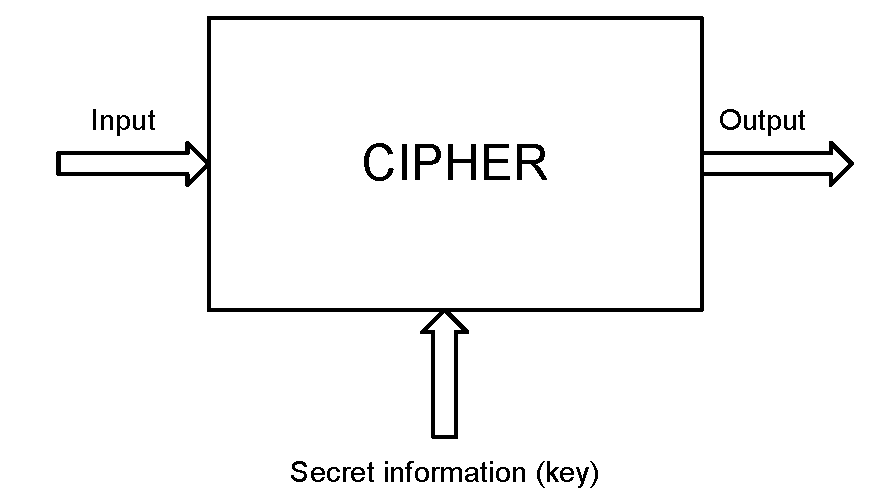
\includegraphics[scale = 0.5]{images/blackbox.pdf}
\end{figure}

\end{frame}

\begin{frame}
	\frametitle{Information Leakage}
In reality, it's hard to prevent additional information from being leaked at runtime.
\begin{figure}
\centering
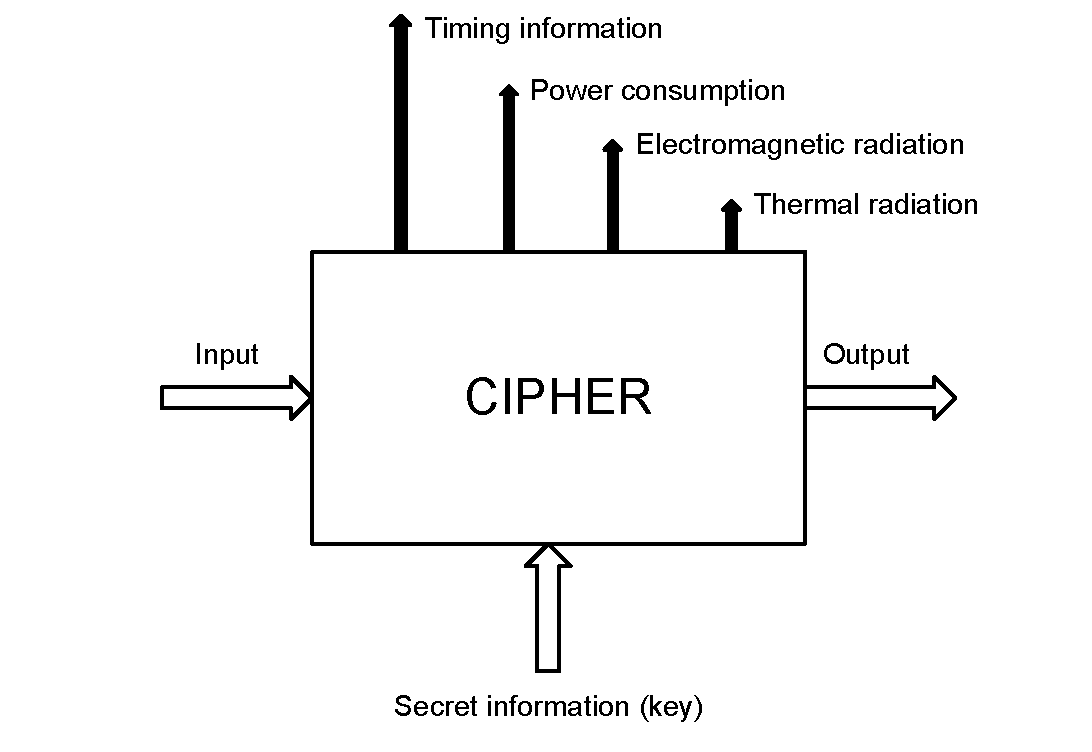
\includegraphics[scale = 0.5]{images/leaked.pdf}
\end{figure}
	
\end{frame}

\begin{frame}
	\frametitle{Side Channel Attacks}
	\textbf{Definition}: Any attack on a cryptosystem using information leaked given off as a byproduct of the physical implementation of the cryptosystem, rather than a theoretical weakness (TODO: CITE jbonneau), is a \emph{side channel attack}.
	\medskip
	We focus on \textbf{timing attacks} for \textbf{software implementations} of AES.
\end{frame}

\section{History of Timing Attacks}
\begin{frame}
	\frametitle{History of Timing Attacks on Cryptographic Primitives}
	\begin{itemize}
		\item LIST OF PAPERS FROM BONNEAU HISTORY
	\end{itemize}
\end{frame}

\begin{frame}
	\frametitle{Timing Attacks on AES}
	\begin{itemize}
		\item Rijndael was deemed not susceptible to timing attacks in the AES contest
		\item AES targeted attacks can be \emph{statistical} (BERNSTEIN)
		\begin{itemize}
			\item Observation: The entire encryption time can be affected
			\item Step 1: 
			\item Step 2: 
		\end{itemize}
		\item Or they can be more targeted
		\begin{itemize}
			\item Exploit relationships between secret information of the primitive and known data.
		\end{itemize}
	\end{itemize}
\end{frame}

\section{Cache Timing Attacks}
\begin{frame}
	\frametitle{Cache Memory}
	TODO: how it's arranged, lines, and whatnot...

$\langle l_i \rangle = \langle l_j \rangle$ are the lower bits of the data entry (data is put into cache based on its MSbits)
\end{frame}

\begin{frame}
	\frametitle{Cache Collisions Reveal Weaknesses}
	Let $T_E(K, P)$ be the encryption time for a plaintext $P$ using key $K$. 
	Let $\bar{T}_E(K)$ be the $\frac{1}{n}\sum_{i = 1}^{n}T_E(K, P_i)$, where $P_i$ is a random plaintext from $\{0|1\}^{128}$.

	\medskip

	\textbf{Cache-Collision Assumption \cite{bonneau}}. For any pair of table lookups $i, j$, given
a large enough number of \emph{random} AES encryption that use the \emph{same key}, $\bar{T}_E(K)$ will
be lower when $\langle l_i \rangle = \langle l_j \rangle$ than when $\langle l_i \rangle \not= \langle l_j \rangle$

	\medskip
	
	Note: The table lookup indices must be \emph{independent} for random plaintexts.
\end{frame}

\begin{frame}
	\frametitle{Cache Collisions (cont'd)}
	Let $a$ and $b$ be two memory addresses looked up in memory. Let $\langle a \rangle$ and $\langle b \rangle$ 
	denote the MSBs of $a$ and $b$, respectively. 
	\begin{itemize}
		\item Cache memory is organized into \emph{lines}
		\begin{itemize}
			\item MSB is mapped to the cache line index, LSB is mapped to the line (block) offset
		\end{itemize}
		\item Reads on $a$ and $b$ cause a collision if $\langle a \rangle = \langle b \rangle$ (assuming other memory reads
		have not evicted (or invalidated) $a$ or $b$ from the cache. 
		\item If $\langle a \rangle \not= \langle b \rangle$ then a cache collision \emph{might} occur.
		\item We cannot say for certain whether or not the lower LSBs are equivalent...
	\end{itemize}
\end{frame}

\begin{frame}
	\frametitle{Attacks from Cache Collisions}
	\begin{center}
	That's it! We may not build an attack based on this result.
	\end{center}
\end{frame}

\section{Cache Timing Attacks on AES}
\subsection{LUT-Based Implementations of AES}
\begin{frame}
	\frametitle{LUT-Based Implementations}
	Let $X^i$ be the state of AES at round $i$. With the exception of $i = 10$, we have:
\begin{align*}
X^{i+1} = \{ & T_0[x_0^i] \oplus T_1[x_5^i] \oplus T_2[x_{10}^i] \oplus T_3[x_{15}^i] \oplus \{k_0^i, k_1^i, k_2^i, k_3^i\}, \\
& T_0[x_4^i] \oplus T_1[x_{9}^i] \oplus T_2[x_{14}^i] \oplus T_3[x_3^i] \oplus \{k_4^i, k_5^i, k_6^i, k_7^i\}, \\
& T_0[x_8^i] \oplus T_1[x_{13}^i] \oplus T_2[x_2^i] \oplus T_3[x_7^i] \oplus \{k_8^i, k_9^i, k_{10}^i, k_{11}^i\}, \\
& T_0[x_{12}^i] \oplus T_1[x_1^i] \oplus T_2[x_6^i] \oplus T_3[x_{11}^i] \oplus \{k_{12}^i, k_{13}^i, k_{14}^i, k_{15}^i\}\}
\end{align*}
\end{frame}

\subsection{First Round Attack}
\begin{frame}
	\frametitle{First Round}
	TODO: image of AES lookup after first round
	\begin{itemize}
		\item First round: $x_i^{0} = p_i \oplus k_i$
		\item With the T-box implementation, $x_0^0$, $x_4^0$, $x_8^0$, and $x_{12}^0$ are 
		used as indices into $T_0$
		\item If we are looking for cache collisions, we must consider input bytes of the same ``family'' 
		(i.e. incides into the same T-box)
	\end{itemize}
	\begin{center}
		\langle x_i^0 \rangle = \langle x_j^0 \rangle & \Rightarrow \\
		& \langle p_i \rangle \oplus \langle k_i \rangle = \langle p_j \rangle \oplus \langle k_j \rangle \Rightarrow \\
		& \langle p_i \rangle \oplus \langle p_j \rangle = \langle k_i \rangle \oplus \langle k_j \rangle \Rightarrow
	\end{center}
\end{frame}

\begin{frame}
	\frametitle{First Round Attack Algorithm}
	\begin{numberedAlg}[FirstRoundAttack($N_s$)]
	\label{eea}
	\begin{algorithmic}[1]
		\State $n \gets 2^8 - 1$
		\State $T \gets$ array$[0 \dots n,1 \dots n, 0 \dots n]$
		\For {$i = 0 \to N_s}
			\State $P \gets RandomBytes(16)$
			\State $start \gets time()$
			\State $C \gets E_K(P)$
			\State $end \gets time(), tt \gets (start - end)$
			\State $t[i,j,\langle p_i \rangle \oplus \langle p_j \rangle] \gets t[i,j,\langle p_i \rangle \oplus \langle p_j \rangle] + tt$
		\EndFor
		\State $t[i,j,\langle p_i \rangle \oplus \langle p_j \rangle] \gets t[i,j,\langle p_i \rangle \oplus \langle p_j \rangle] / N_s$
		\State $mi,mj \gets min(t)$ \Comment{Use t-test if necessary}
		\State $\langle k_{mi} \rangle \oplus \langle k_{mj} \rangle \gets \langle p_{mi} \rangle \oplus \langle p_{mj} \rangle$
	\end{algorithmic}
	\end{numberedAlg} 
\end{frame}

\begin{frame}
	\frametitle{First Round Attack Algorithm (cont'd)}
	TODO: show how selection of the six equations works... circle relations on the matrix...
	0/4, 0/8, 0/12, 4/8, 4/12, 8/12 (six for each T-box), can try to solve from there
	Limitation: We only know the upper bytes, we cna't figure out the block offset...
\end{frame}

\subsection{Last Round Attack}
\begin{frame}
	\frametitle{The Last Round}
	When $i = 10$, the lookup table is just the S-box $S$. At this point, the ciphertext $C$ is:
\begin{align*}
C = \{ & S[x_0^{10}] \oplus k_0^{10}, S[x_5^{10}] \oplus k_1^{10}, S[x_{10}^{10}] \oplus k_2^{10}, S[x_{15}^{10}] \oplus k_3^{10}, \\
& S[x_4^{10}] \opus k_5^{10}, S[x_9^{10}] \oplus k_6^{10}, S[x_{14}^{10}] \oplus k_7^{10}, S[x_3^{10}] \oplus k_7^{10}, \\
& S[x_8^{10}] \oplus k_8^{10}, S[x_{13}^{10}] \oplus k_9^{10}, S[x_2^{10}] \oplus k_{10}^{10}, S[x_7^{10}] \oplus k_{11}^{10}, \\
& S[x_{12}^{10}] \oplus k_{12}^{10}, S[x_{1}^{10}] \oplus k_{13}^{10}, S[x_6^{10}] \oplus k_{14}^{10}, S[x_{11}^{10}] \oplus k_{15}^{10}\} 
\end{align*}
\end{frame}

\begin{frame}
	\frametitle{Final Round}
\end{frame}

\begin{frame}
	\frametitle{Final Round Attack Algorithm}
\end{frame}

\begin{frame}
	\frametitle{Timing Attack Countermeasures}
	\begin{itemize}
		\item Masking...
	\end{itemize}
\end{frame}	

\begin{comment}
\begin{figure}
\centering
\includegraphics[scale = 0.6]{images/sub_layer.jpg}
\end{figure}
\end{comment}

\end{document}
